% Bluetooth
\subsection{Bluetooth}%
\label{sec:bluetooth}
Bluetooth is a ubiquituous radio-frequency technology (2.4 GHz) for wireless
communication, generally at short distances. Bluetooth is managed by the
\gls{sig} and the current version of the standard
is 5.0. Starting from version 4.0, also known as \gls{ble}, power consumption
was minimised, making it suitable for embedded and \gls{iot}
applications. Bluetooth is a full protocol stack, illustrated in
Fig.~\ref{fig:ble-stack}, comprising the controller, the host device and the
applications interacting with the device. The \gls{hci} layer enables the host
device to interface the controller, required for low-level operations such as
asynchronous device discovery or reading radio signal intensity. The host
provides profiles to the external applications, easing the interaction betwen
device and applications.
%
\begin{figure}[!hbt]
\centering
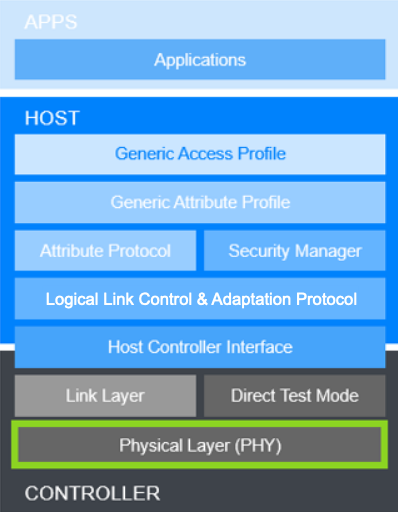
\includegraphics[width=0.45\textwidth]{./img/ble-stack.png}
  \caption{Bluetooth 5.0 protocol stack}%
\label{fig:ble-stack}
\end{figure}
%
Conceptually, Bluetooth is very similar to \gls{tcpip} stack. Both are part of
the network programming class and share the same principles of communication and
data exchange between devices. The difference is that Bluetooth was designed for
short distance communication, whereas the internet programming does not share
this concern. This affects how two devices detect each other initially and how
they establish the initial connection. From that moment on, the procedure is
similar to the \gls{tcpip} stack (see Fig.~\ref{fig:bt-outgoing} and
Fig.~\ref{fig:bt-incoming}).
%
\subsubsection{Establishing a connection}%
\label{sec:bt-establish-conn}
Establishing a connection depends if the device in analysis is trying to
establish an \uline{outgoing} or \uline{incoming} connection. Basically, for the
former case the device sends the first data packet to start the communication,
and for the latter the device receives the first data packet. The devices that
initiate \uline{outgoing} connections must choose a target device and a
transport protocol, before establishing the connection and exchange data. The
devices that initiate \uline{incoming} connections must select a transport
protocol and then \textit{listen} for incoming connections, before establishing
the connection and exchange data~\cite{huang2007bluetooth}.

Figures~\ref{fig:bt-outgoing} and~\ref{fig:bt-incoming} illustrate this concept,
comparing network, internet and bluetooth programming for outgoing and incoming
connections, respectively. For outgoing connections, only the two first steps
(choosing a target device, transport protocol and port number) are different;
after the connection is established, the process is similar. For incoing
connections the procedures are even more similar, with the major difference that
port numbers are dynamically assigned for Bluetooth programming. The procedures
for programming outgoing and incoming connections are presented next.

\uline{Outgoing connection programming procedure}:
\begin{enumerate}
\item Choose a target device
\item Choose a transport protocol and port number
\item Establish a connection
\item Exchange data
\item Disconnect
\end{enumerate}

\uline{Incoming connection programming procedure}:
\begin{enumerate}
\item Choose a transport protocol and port number
\item Reserve local resources and go into listening mode
\item Wait and accept incoming connections
\item Exchange data
\item Disconnect
\end{enumerate}
% Outgoing connections
\begin{figure}[!hbt]
\centering
    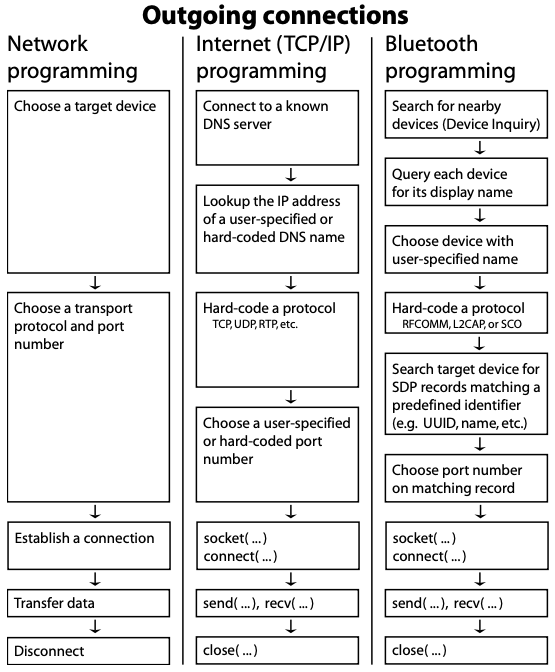
\includegraphics[width=0.47\textwidth]{./img/bt-outgoing.png}
  \caption{Comparison of Network, Internet and Bluetooth programming for
    outgoing connections (withdrawn from~\cite{huang2007bluetooth})}%
\label{fig:bt-outgoing}
\end{figure}
%
%
\begin{figure}[!hbt]
\centering
    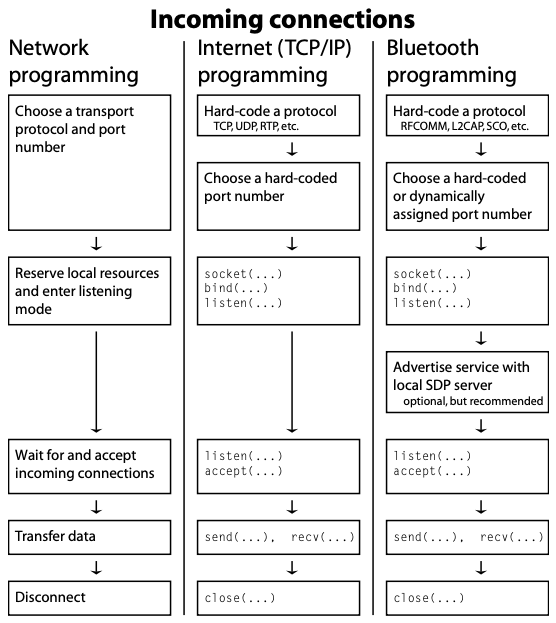
\includegraphics[width=0.47\textwidth]{./img/bt-incoming.png}
  \caption{Comparison of Network, Internet and Bluetooth programming for
    incoming connections (withdrawn from~\cite{huang2007bluetooth})}%
\label{fig:bt-incoming}
\end{figure}
%
\subsubsection{Selecting a target device}%
\label{sec:bt-target-device}
Every Bluetooth chip manufactured has a 48-bit unique address --- BT address ---
identical to the \gls{mac1} for Ethernet protocol, acting as the basic addressing
unit for Bluetooth programming.

The Bluetooth device must know the target device address to
communicate. However, the client application does not need to know \textit{a
  priori} the target address: the end-user provides a user-friendly name ---
\textit{device name} --- and the client translate this to the physical address
when searching for nearby devices. The \textit{device name} may not be unique,
but the address must be.

In the device name lookup process, the device searches for the nearby devices by
inquiring each device individually and compiling a list with their addresses,
which is generally slow. A
Bluetooth device does not announce its presence to other devices; it must start
a device discovery process --- \textit{Device Inquiry} --- to detect them. In
the \textit{Device Inquiry} process the device broadcast a discovery message and
waits for replies. Each reply consists of the physical address of the device and
of an integer identifier the class of the device (e.g., smartphone, headset,
etc.). More detailed information, such as the device name, may be obtained by
contacting each discovered device individually. Additionally, for privacy and
power consumption reasons, the device may choose not to respond to device
inquiries or connections attempts.
%
\subsubsection{Transport protocols}%
\label{sec:bt-transport-protocols}
%
Different applications have different needs, thus the need for different
transport protocols. The two factors that distinguish these protocols are
\textit{guarantees} and \textit{semantics}. The guarantees of a protocol state
how hard it tries to deliver a packet sent by the application, yielding:
\emph{robust} protocols, like \gls{tcp}, which ensures that all sent packets are
delivered or terminates the connection; \emph{best-effort} protocols, like \gls{udp},
which makes a reasonable attempt at delivering transmitted packets, but ignores
its failure. The semantics of a protocol concerns if it distinguishes between
datagrams beginning and end, and can be either packet-based (UDP) or
streams-based (TCP).

Bluetooth contains four essential transport protocols, namely, by relevance
order:
\begin{enumerate}
\item \gls{rfcomm}: reliable and stream-based protocol, which emulates well
  serail ports. It allows only 30 open ports per device and it is the most
  frequently used protocol.
\item \gls{l2cap}: packet-based protocol which can be configured for several
  levels of reliability, imposing delivery order, unlike \gls{udp}. It
  encapsulates the \gls{rfcomm} connection.
\item \gls{acl}: It is not explicitly used, but it encapsulates \gls{l2cap}
  connections. Two Bluetooth devices may have, at most, one \gls{acl} connection
  between them, which is used to transport all \gls{rfcomm} and \gls{l2cap}
  traffic.
\item \gls{sco}: best-effort and packet-based protocol, which is used
  exclusively to transmit voice-quality audio at precisely 64 Kb/s.
\end{enumerate}
The summary of Bluetooth transport protocols is illustrated in
Fig.~\ref{fig:bt-transport-protocols-summary}, where is visibly the connection
encapsulation. Two Bluetooth devices may have, at most, one \gls{acl} and \gls{sco} connection
between them, whereas the number of \gls{rfcomm} and \gls{l2cap} active
connection is limited only by the number of available ports.
% Transport protocols summary
\begin{figure}[!hbt]
\centering
    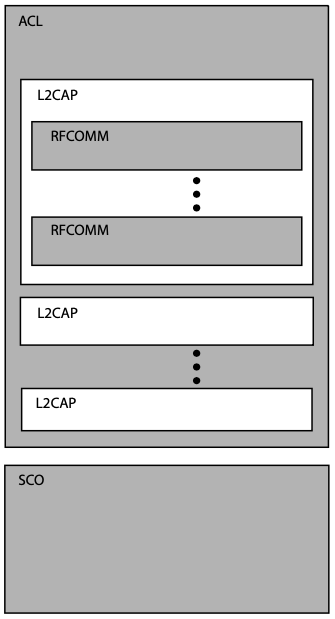
\includegraphics[width=0.3\textwidth]{./img/bt-transport-protocols-summary.png}
  \caption{Most relevant Bluetooth transport protocols (withdrawn from~\cite{huang2007bluetooth})}%
\label{fig:bt-transport-protocols-summary}
\end{figure}
\newpage
%
\subsubsection{Port Numbers}%
\label{sec:bt-port-nrs}
%
A port is used to enable multiple applications on the same device to use the
same transport protocol. Bluetooth uses a slightly different terminology: for
\gls{l2cap}, ports are called \gls{psm} (range of 1--32767); for
\gls{rfcomm}, ports are called channels (range of 1--30).

Some protocols have a set of reserved/well-known ports, intended for
specific usage. \gls{l2cap} reserves ports 1--1023
for standardized usage (e.g., \gls{sdp} uses port 1), whereas \gls{rfcomm} does
not have reserved ports, given its small number.
\subsubsection{Service discovery}%
\label{sec:bt-service-discovery}
%
For a client application to initiate a outgoing connection it must know in which
port the server application is listening. If the application is standard, then a
reserved port is used. The traditional approach for Internet programming is
hardcoding the same port number at both client and server: when the connection
is established, the server listens on that part and the client connects to
it. However, the static port definition is cumbersome and prevents two server
applications from using the same port.

Bluetooth tries to solve this problem by introducing \gls{sdp}, as illustrated
in Fig.~\ref{fig:bt-sdp-operation}:
\begin{enumerate}
\item Each device keeps an \gls{sdp} server listening on a well-known port.
\item When the server application is executed, it stores a description of itself
  and a port number in the \gls{sdp} server on the local device.
\item Then, when a remote cliente application connects for the first time to the
  device, it provides a description of the service it is searching for, and the
  \gls{sdp} server returns a list of all corresponding services with the
  respective associated port numbers.
\end{enumerate}
% Comparison between connection establishments
\begin{figure}[!hbt]
\centering
    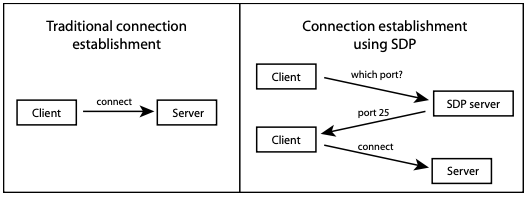
\includegraphics[width=0.6\textwidth]{./img/bt-sdp-operation.png}
  \caption{Comparison between traditional connection establishment (internet)
    and using SDP (Bluetooth) (withdrawn from~\cite{huang2007bluetooth})}%
\label{fig:bt-sdp-operation}
\end{figure}
\subsubsection{Host Controller Interface --- HCI}%
\label{sec:bt-hci}
%
The \gls{hci} defines how a host (e.g., a computer) interacts and communicates
with the local Bluetooth adapter (the controller). All communications between
these two agents are encapsulated in \gls{hci} packets, of four different kinds:
\begin{enumerate}
\item \uline{Command}: sent from the host to the local adapter to control it,
  which can be used for starting a device discovery, connecting to a remote
  device, adjusting the connection parameters, amongst others.
\item \uline{Event}: generated by the local adapter and sent to the host when an
  event of interest occurs, for example, device detected, connection
  established, etc.
\item \uline{ACL data}: encapsulates data to send ou received from a remote
  Bluetooth device. In this sense, the \gls{hci} is a transport protocol for all
  transport protocols (\gls{acl},\gls{l2cap}, and \gls{rfcomm}). When packets
  arrive to the local adapter, the \gls{hci} headers are removed and the pure
  \gls{acl} packet is transmitted through air.
\item \uline{SCO}
\end{enumerate}

\subsubsection{Development Stacks for Bluetooth}%
\label{sec:bt-hci}
%%% Local Variables:
%%% mode: latex
%%% TeX-master: "../../../dissertation"
%%% End:
A development stack refers to a collection of device drivers, development libraries and
tools provided to enable software developers to create Bluetooth
applications. In most operating systems there is a Bluetooth dominant stack,
easing development, as there is a high level of incompatibility between
Bluetooth development stacks. Since Bluetooth is a communications technology,
the transport protocols supported by each stack are of particular
interest. Occasionaly, wrappers around the developed libraries for a stack are
created to provide a higher abstraction programming interface for Bluetooth, in
languages like Python or Java. The most relevant development stacks and wrappers
are depicted in Fig.~\ref{fig:bt-stacks}.
% Bluetooth stacks
\begin{figure}[!hbt]
\centering
    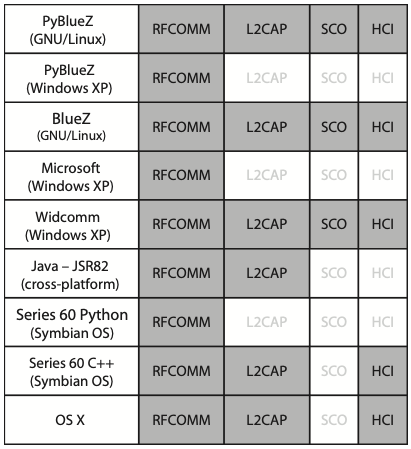
\includegraphics[width=0.4\textwidth]{./img/bt-stacks.png}
  \caption{Most relevant development Bluetooth stacks and wrappers and its
    supported protocols (withdrawn from~\cite{huang2007bluetooth})}%
\label{fig:bt-stacks}
\end{figure}

The Bluetooth development stack selected was \textbf{BlueZ}, since its a
powerful open source stack, included in all major GNU/Linux distributions and
with extensive \gls{api}~s, supporting a extensive set of protocols which
enables to fully explore the Bluetooth local resources. The \gls{rfcomm},
\gls{l2cap}, and \gls{sco} protocols are acessed using the standard sockets
interface and the \gls{hci} is more conveniently used through the provided
wrappers around the several \gls{hci} commands and events.
%